\documentclass[a4paper,14pt]{extarticle} 
\usepackage[a4paper,top=1.5cm, bottom=1.5cm, left=2cm, right=1cm]{geometry}
%\usepackage[T2A]{fontenc}
%\usepackage[english, russian]{babel}
\usepackage{graphicx}
\DeclareGraphicsExtensions{.pdf,.png,.jpg}

\usepackage{fontspec}
\setmainfont{Times New Roman}
\setsansfont{FreeSans}
\setmonofont{FreeMono}
\renewcommand{\baselinestretch}{1.5}
\usepackage{polyglossia}
\setdefaultlanguage{russian}
\setotherlanguages{english,russian}
\usepackage{setspace}
\usepackage[many]{tcolorbox}
\usepackage{listings}
\usepackage{xcolor}

\definecolor{codegreen}{rgb}{0,0.6,0}
\definecolor{codegray}{rgb}{0.5,0.5,0.5}
\definecolor{codepurple}{rgb}{0.58,0,0.82}
\definecolor{backcolour}{rgb}{0.95,0.95,0.92}

\lstdefinestyle{mystyle}{
    backgroundcolor=\color{backcolour},   
    keywordstyle=\color{magenta},
    numberstyle=\tiny\color{codegray},
    stringstyle=\color{codepurple},
    basicstyle=\ttfamily\footnotesize,
    breakatwhitespace=false,         
    breaklines=true,                 
    captionpos=b,                    
    keepspaces=true,                 
    numbers=left,                    
    numbersep=5pt,                  
    showspaces=false,                
    showstringspaces=false,
    showtabs=false,                  
    tabsize=2
}

\lstset{style=mystyle}

\begin{document}
    \begin{center}
        \thispagestyle{empty}
        \begin{singlespace}
        МИНИСТЕРСТВО ЦИФРОВОГО РАЗВИТИЯ, СВЯЗИ И МАССОВЫХ КОММУНИКАЦИЙ РОССИЙСКОЙ ФЕДЕРАЦИИ

        ФЕДЕРАЛЬНОЕ ГОСУДАРСТВЕННОЕ БЮДЖЕТНОЕ ОБРАЗОВАТЕЛЬНОЕ

        УЧРЕЖДЕНИЕ ВЫСШЕГО ОБРАЗОВАНИЯ

        «САНКТ-ПЕТЕРБУРГСКИЙ ГОСУДАРСТВЕННЫЙ УНИВЕРСИТЕТ ТЕЛЕКОММУНИКАЦИЙ ИМ. ПРОФ. М.А. БОНЧ-БРУЕВИЧА»

        (СПбГУТ)
        \end{singlespace}
        \vspace{-1ex}
        \rule{\textwidth}{0.4pt}
        \vspace{-5ex}

        Факультет \underline{Инфокоммуникационных сетей и систем}

        Кафедра \underline{Защищенных систем связи}
        \vspace{10ex}

        \textbf{Лабораторная работа №6}

    \end{center}
    \vspace{4ex}
    \begin{flushright}
    \parbox{10 cm}{
    \begin{flushleft}
        Выполнили студенты группы ИКТЗ-83:

        \underline{Громов А.А., Миколаени М.С., Мазеин Д.С.} \hfill \rule[-0.85ex]{0.1\textwidth}{0.6pt}

        \footnotesize \textit{ (Ф.И.О., № группы) \hfill (подпись)} \normalsize

        Проверил:

        \underline{Скорых М.А.} \hfill \rule[-0.85ex]{0.1\textwidth}{0.6pt}

        (\footnotesize \textit{уч. степень, уч. звание, Ф.И.О.) \hfill (подпись)} \normalsize

    \end{flushleft}
    }
    \end{flushright}
    \begin{center}
        \vfill
        Санкт-Петербург

        2021

    \end{center}
    \newpage

    \textbf{Цель лабораторной работы:}
    Повторение основных концепций из курса "Основы построения компьютерных сетей"
    

    \begin{enumerate}
        \item lab 3.1.4
        \begin{itemize}
            \item
                \begin{center}
                    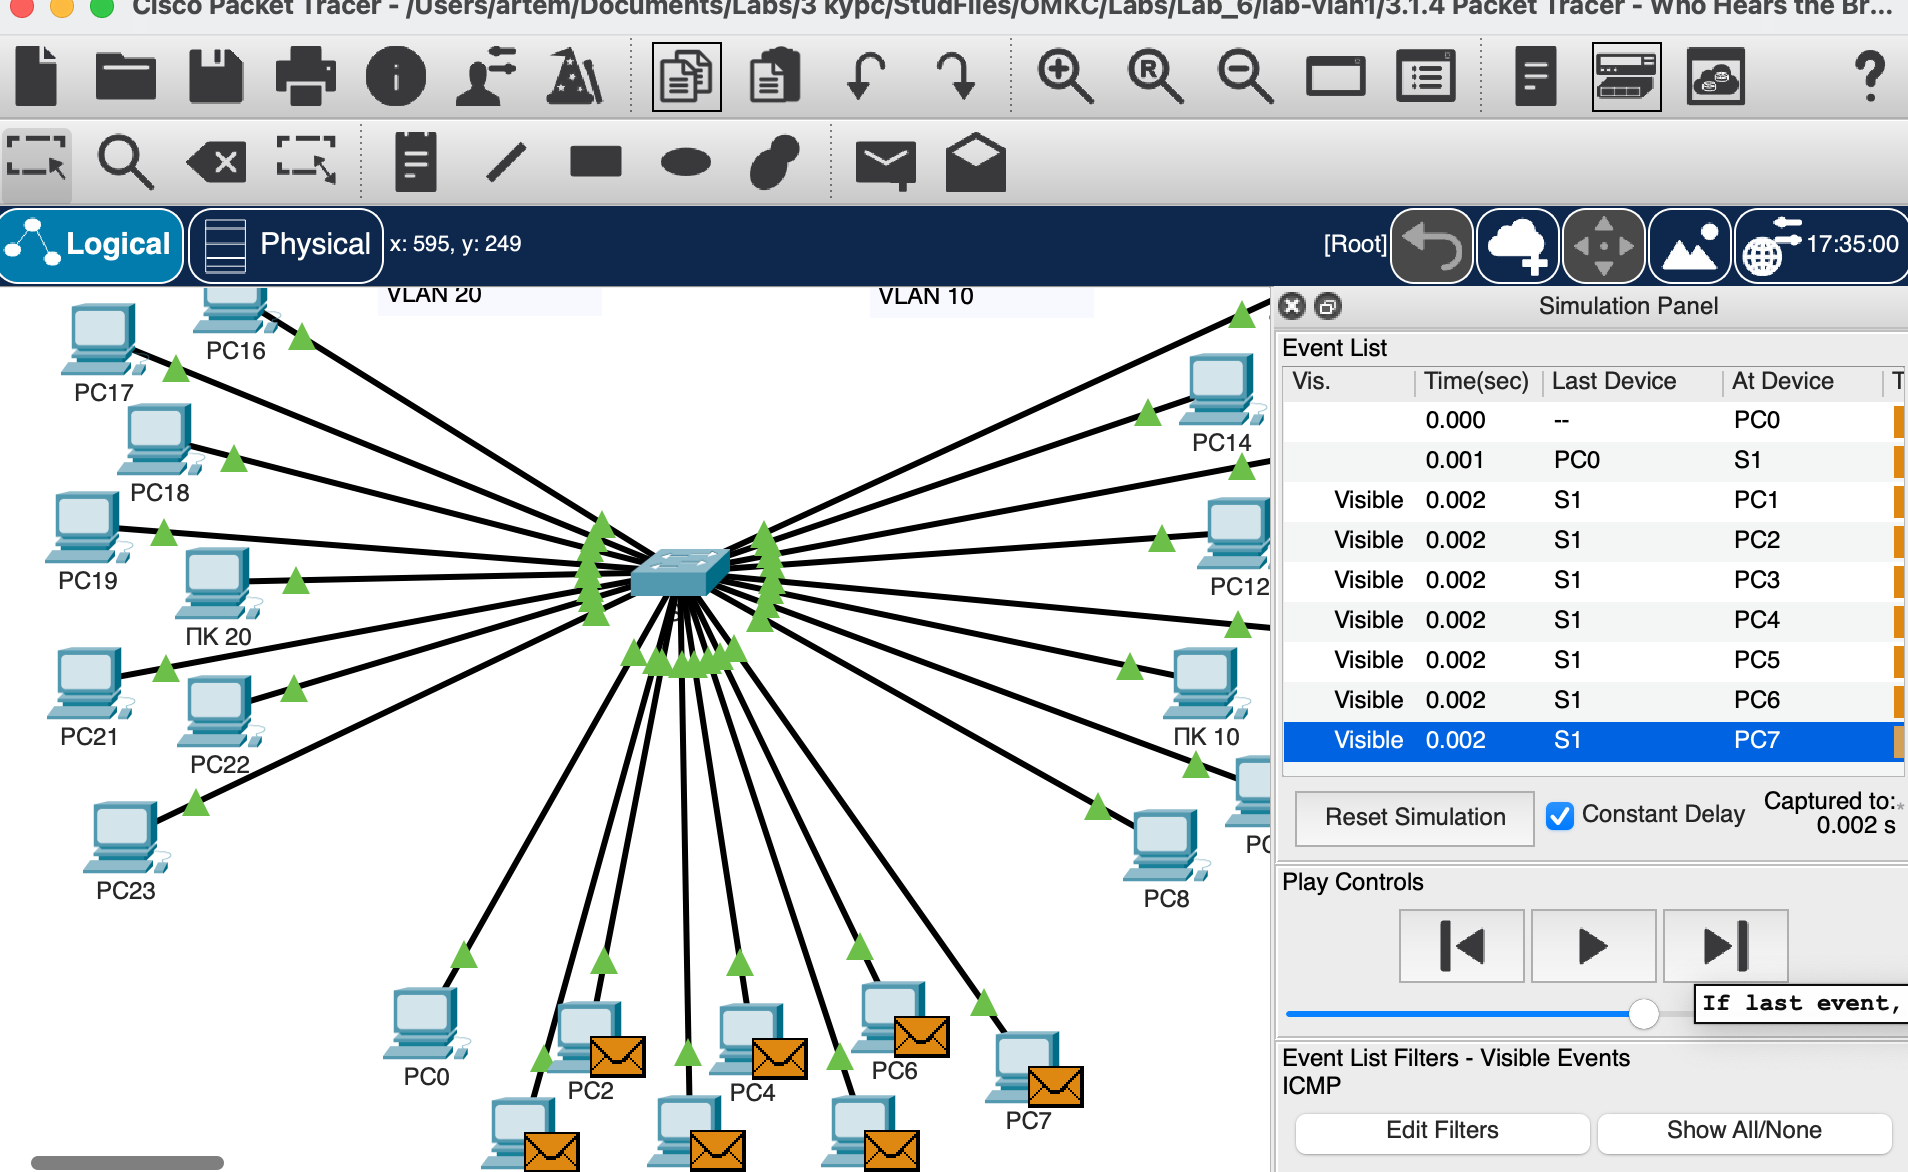
\includegraphics[scale=0.4]{pics/3.1.4_1.png} 
                    Широковещательный запрос
                \end{center} 

            \item \textbf{Назовите не менее трех других доступных приложений.}\par
            HTTP, HTTPS, SSH

            \item \textbf{Если компьютер в сети VLAN 10 отправляет широковещательное сообщение, какие устройства его получат?}\par
            Устройства, которые находятся в VLAN 10.

            \item \textbf{Если компьютер в сети VLAN 20 отправляет широковещательное сообщение, какие устройства его получат?}\par
            Устройства, которые находятся в VLAN 20.

            \item \textbf{Если компьютер в сети VLAN 30 отправляет широковещательное сообщение, какие устройства его получат?}\par
            Устройства, которые находятся в VLAN 30.

            \item \textbf{Что происходит с кадром, отправленным с компьютера сети VLAN 10 на компьютер сети VLAN 30?}\par
            Кадр будет отброшен.

            \item \textbf{Какие порты включаются на коммутаторе, если компьютер, \linebreak подключенный к порту 11, отправляет одноадресное сообщение на компьютер, подключенный к порту 13?}\par
            В передаче будут задействованы порты fa0/11 и fa0/13.

            \item \textbf{Какие порты включаются на коммутаторе, если компьютер, \linebreak подключенный к порту 2, отправляет одноадресное сообщение на \linebreak компьютер, подключенный к порту 23?}\par
            В попытке передачи одноадресного сообщения будут задействованы все порты относящиеся к Vlan источника. Порт получателя задействован не будет.

            \item \textbf{Что представляют собой коллизионные домены на коммутаторе применительно к портам?}\par
            Каждое соединение коммутатора с хостом образует коллизионный домен. То есть в нашем случае их 24.

            \item \textbf{Что представляют собой широковещательные домены на коммутаторе применительно к портам?}\par
            Каждый vlan создает широковещательный домен. То есть в нашем случае их 3. Порты в одном vlan являются частью одного широковещательного домена.

        \end{itemize}
        \newpage
        \item lab 3.2.8
        \begin{itemize}
            \item 
                \begin{center}
                    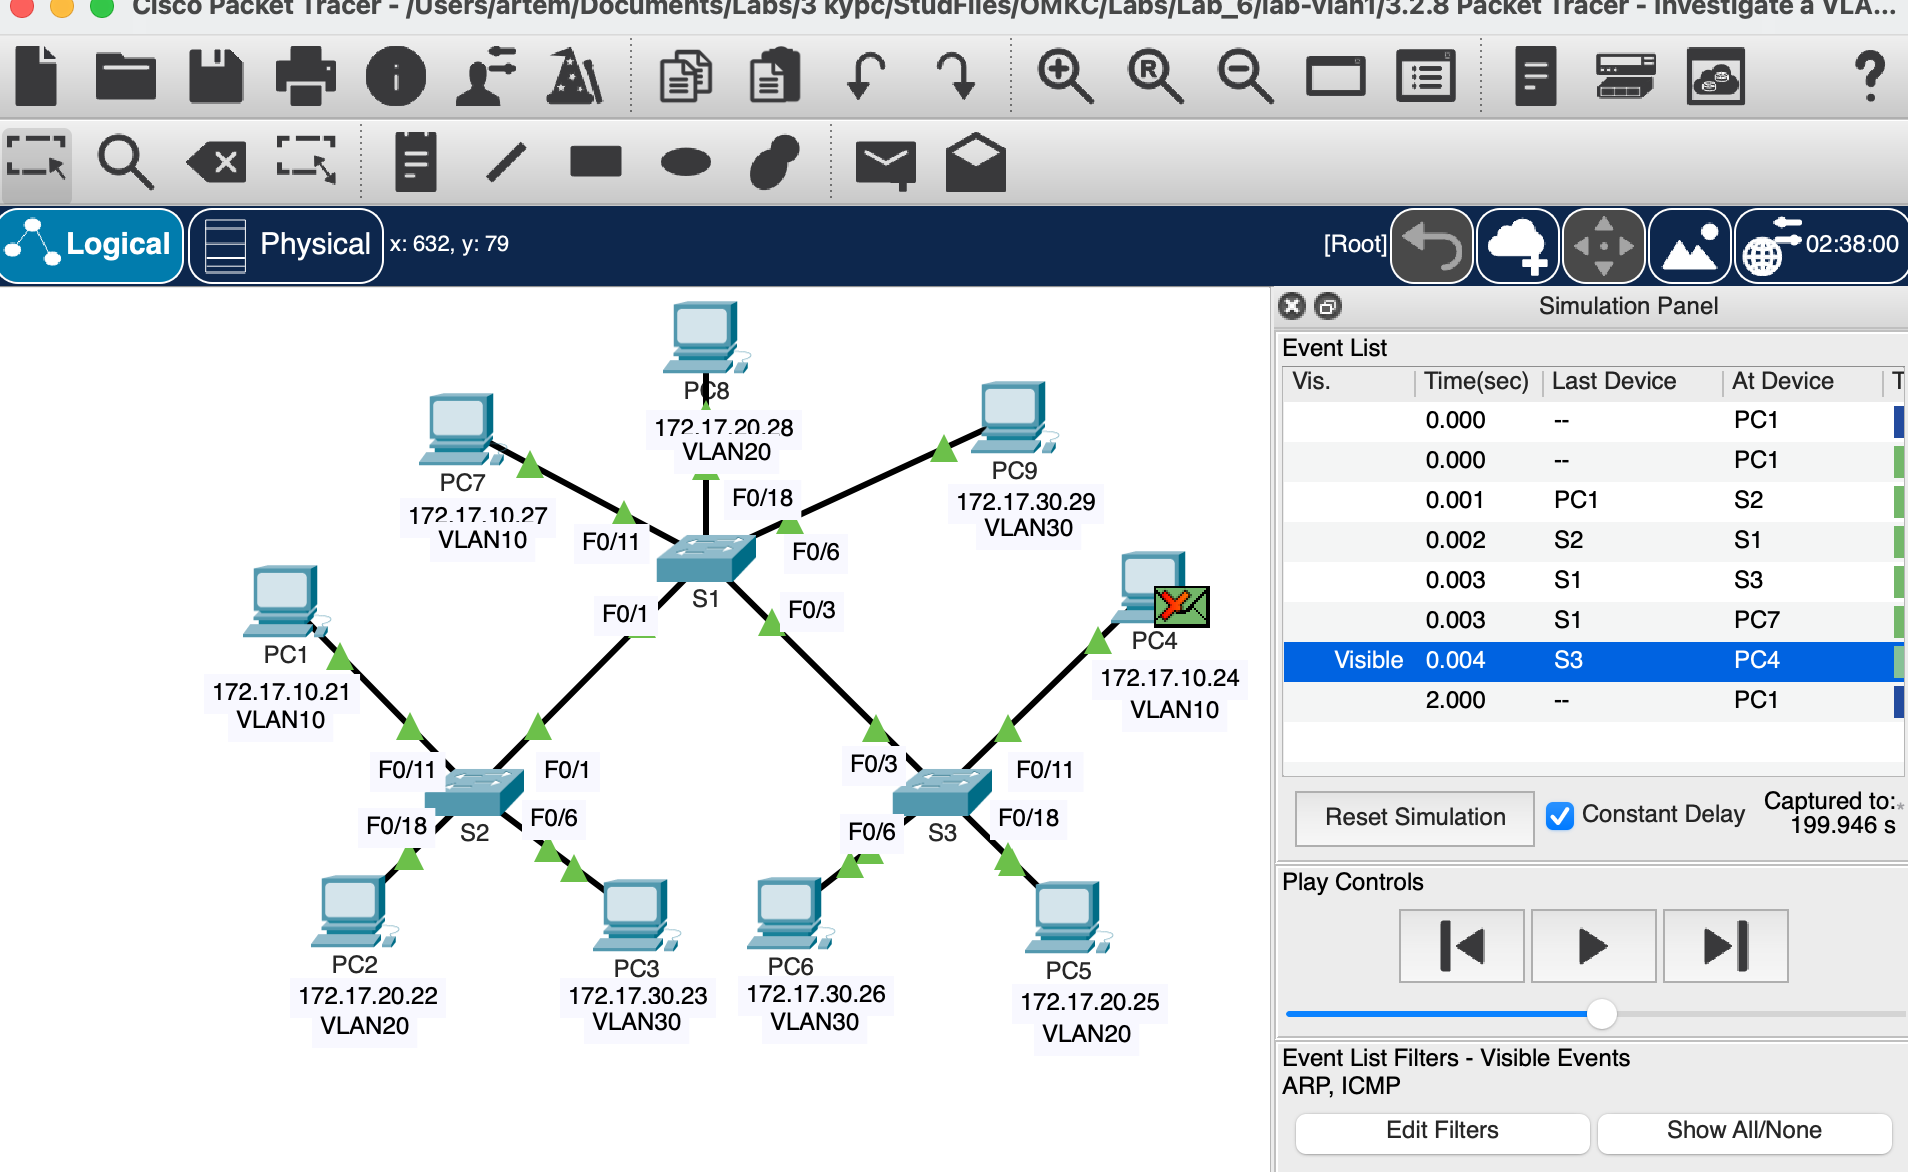
\includegraphics[scale=0.4]{pics/3.2.8_1.png}
                    \singlespacing
                    Попытка сделать ping запрос на PC6(неудачная, так как PC6 в другом vlan)
                \end{center}
            \item 
                \begin{center}
                    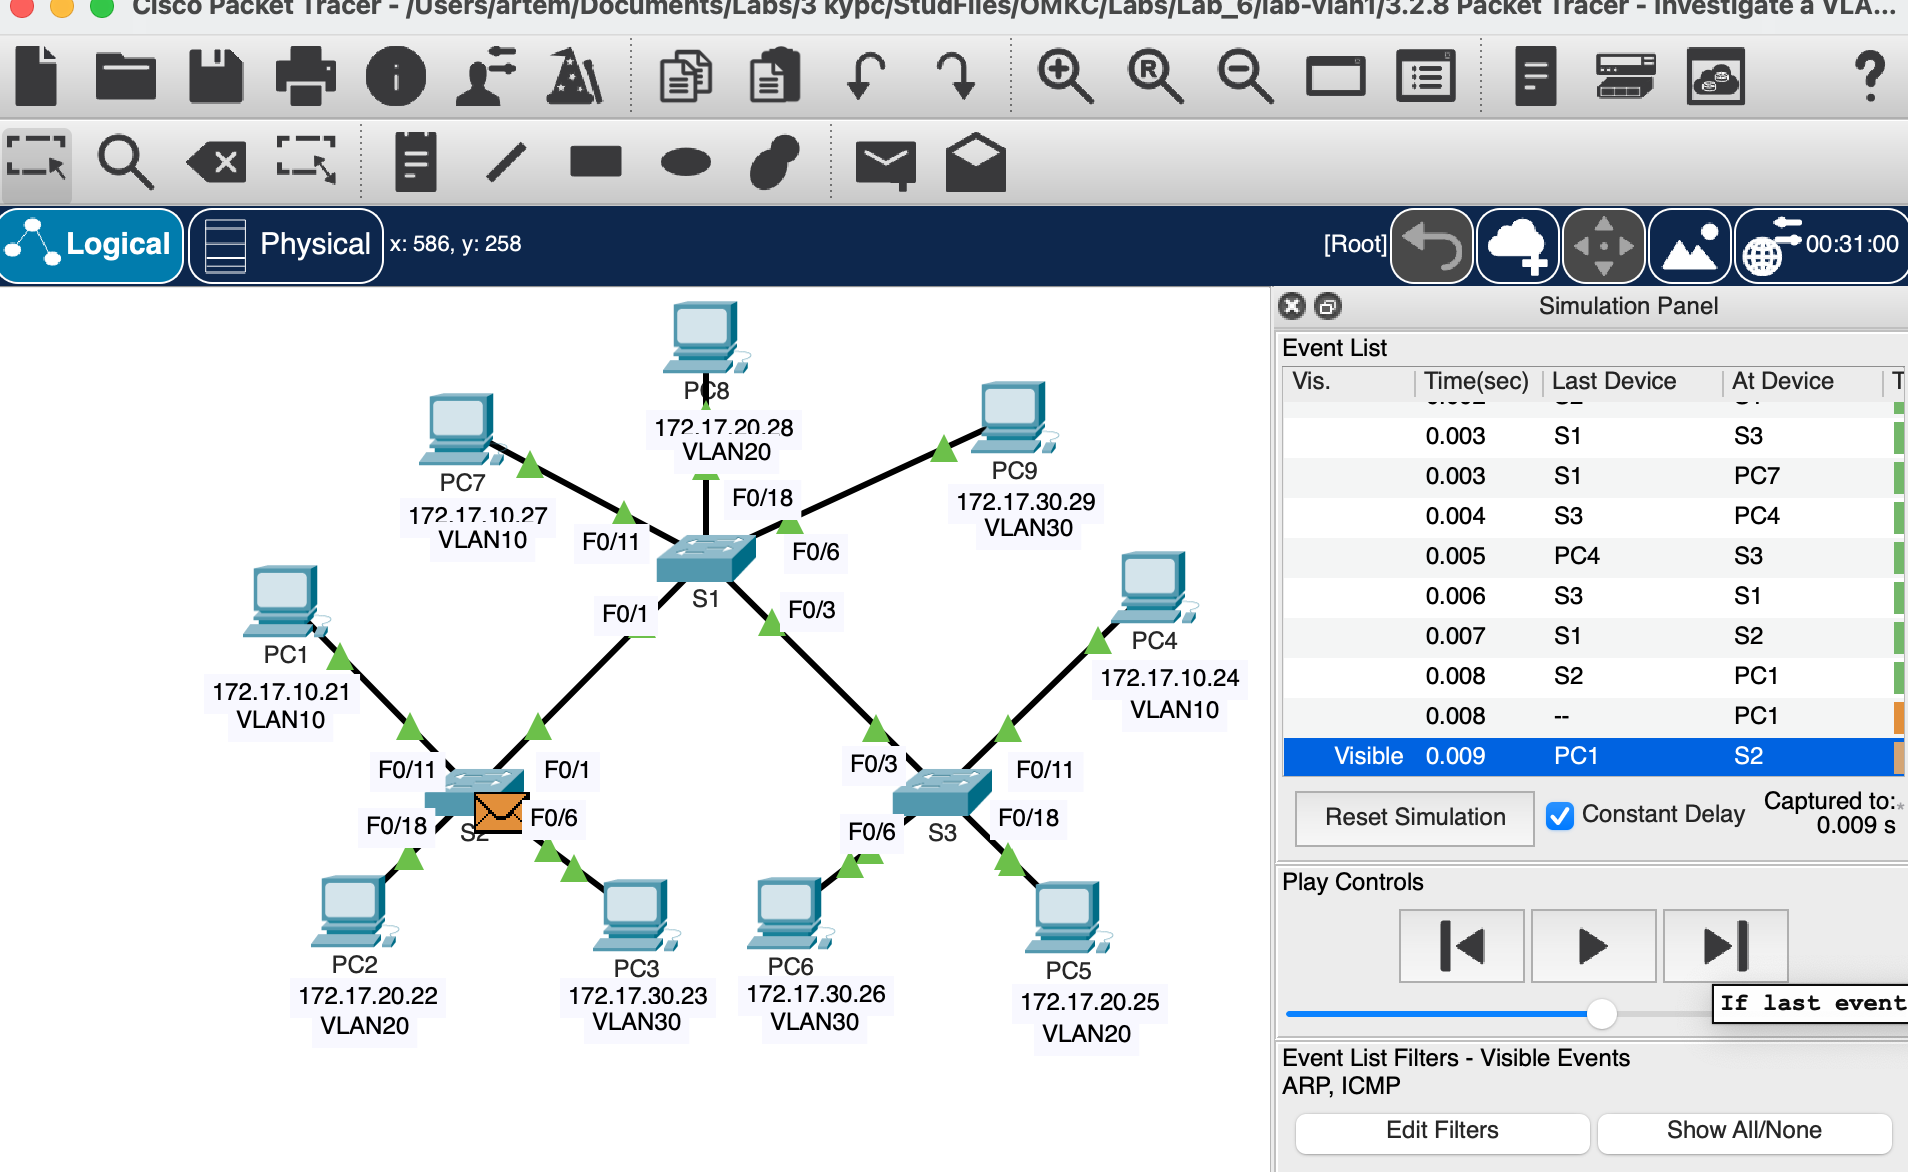
\includegraphics[scale=0.4]{pics/3.2.8_2.png}
                    \singlespacing
                    Попытка сделать ping запрос на PC4(удачно, так как PC1 и PC4 находятся в одном vlan)
                \end{center}
            \item \textbf{Почему коммутатор S1, получив пакет, пересылает его на узел PC7?}\par
            Так как PC7 находится в одном vlan с PC1.

            \item \textbf{Какая команда используется для удаления загрузочной конфигурации на коммутаторах?}\par
            \begin{lstlisting}
erase startup-config
            \end{lstlisting}

            \item \textbf{Где на коммутаторах хранится файл сети VLAN?}\par
            \begin{lstlisting}
flash:/vlan.dat
            \end{lstlisting}

            \item \textbf{С помощью какой команды можно удалить файл сети VLAN на коммутаторах?}\par
            \begin{lstlisting}
delete flash:/vlan.dat
            \end{lstlisting}

            \item \textbf{Если компьютер в сети VLAN 10 отправляет широковещательное сообщение, какие устройства его получат?}\par
               Устройства находящиеся в vlan 10. 

            \item \textbf{Если компьютер в сети VLAN 20 отправляет широковещательное сообщение, какие устройства его получат?}\par
               Устройства находящиеся в vlan 20. 

            \item \textbf{Если компьютер в сети VLAN 30 отправляет широковещательное сообщение, какие устройства его получат?}\par
               Устройства находящиеся в vlan 30. 

            \item \textbf{Что происходит с кадром, отправленным с компьютера сети VLAN 10 на компьютер сети VLAN 30?}\par
                Кадр отбрасывается.

            \item \textbf{Что представляют собой коллизионные домены на коммутаторе применительно к портам?}\par
                Каждое соединение коммутатора с хостом образует коллизионный домен. То есть в нашем случае их 24.

            \item \textbf{Что представляют собой широковещательные домены на коммутаторе применительно к портам?}\par
                Каждый vlan создает широковещательный домен. То есть в нашем случае их 3. Порты в одном vlan являются частью одного широковещательного домена.

        \end{itemize}
        \item lab 3.3.12
        \begin{itemize}
            \item \textbf{Какие преимущества могут предоставить сети VLAN?}
                Они помогут ограничить широковещательный домен до машин из одной сети, так как без vlan широковещательные сообщения получают все пк.
                \begin{center}
                    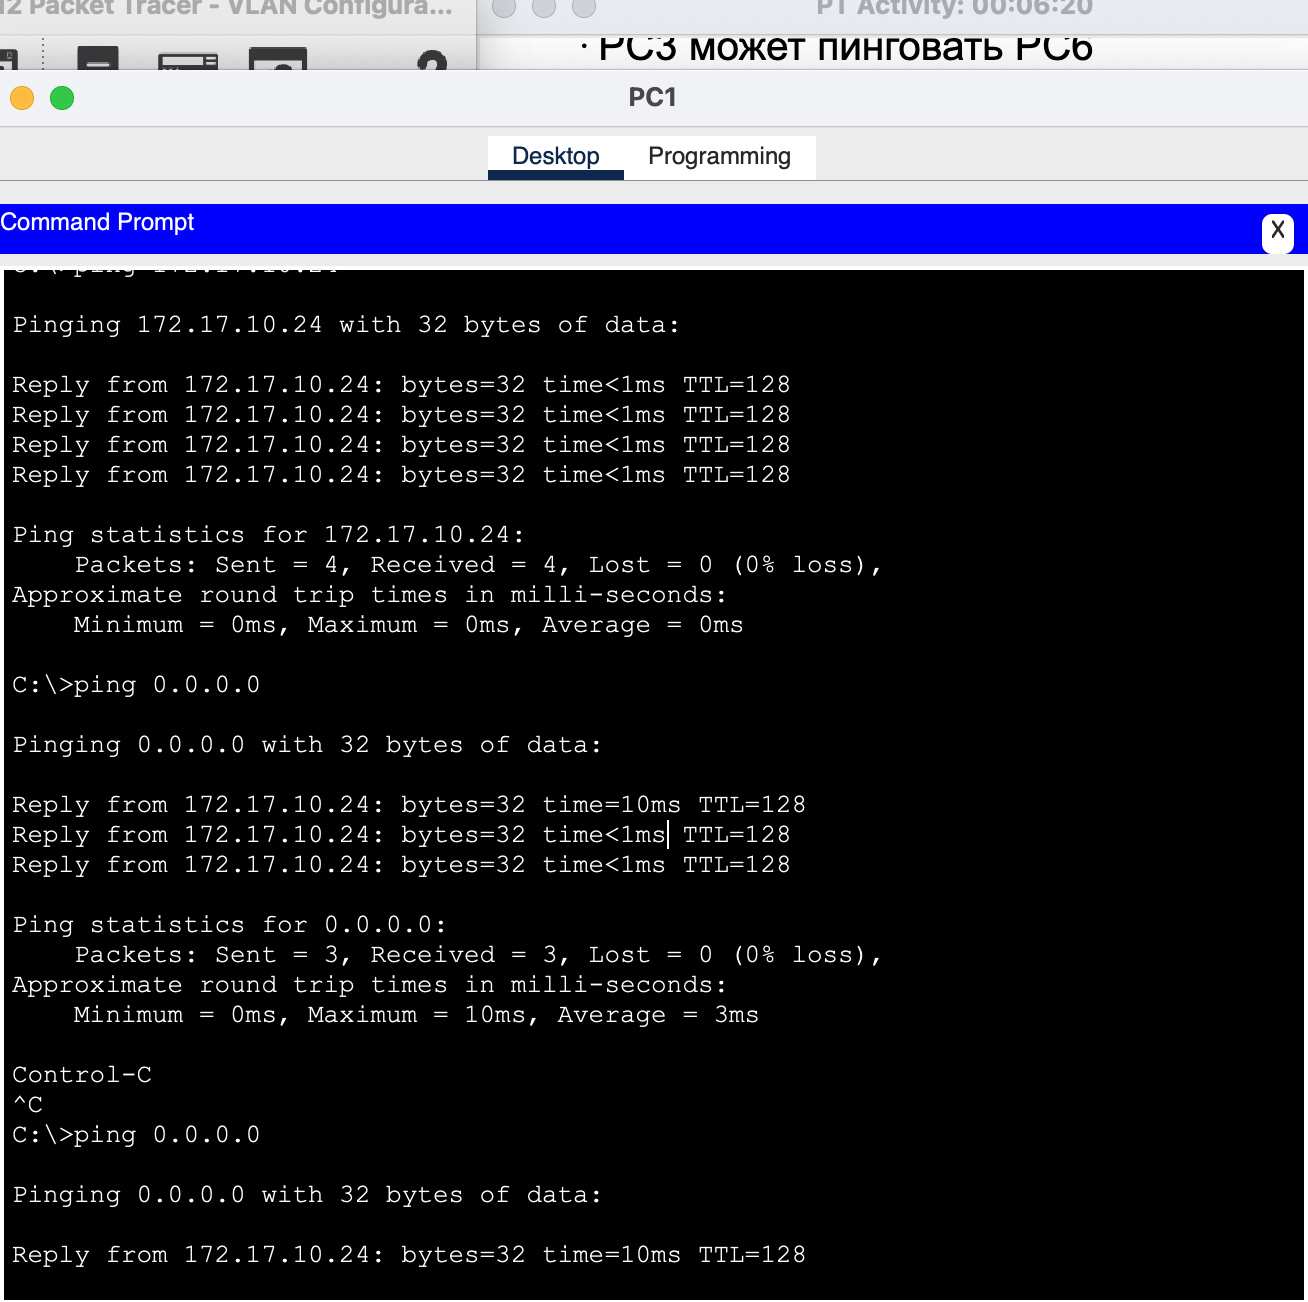
\includegraphics[scale=0.5]{pics/3.3.12_2.png}
                    
                    Делаем широковещательный запрос.
                    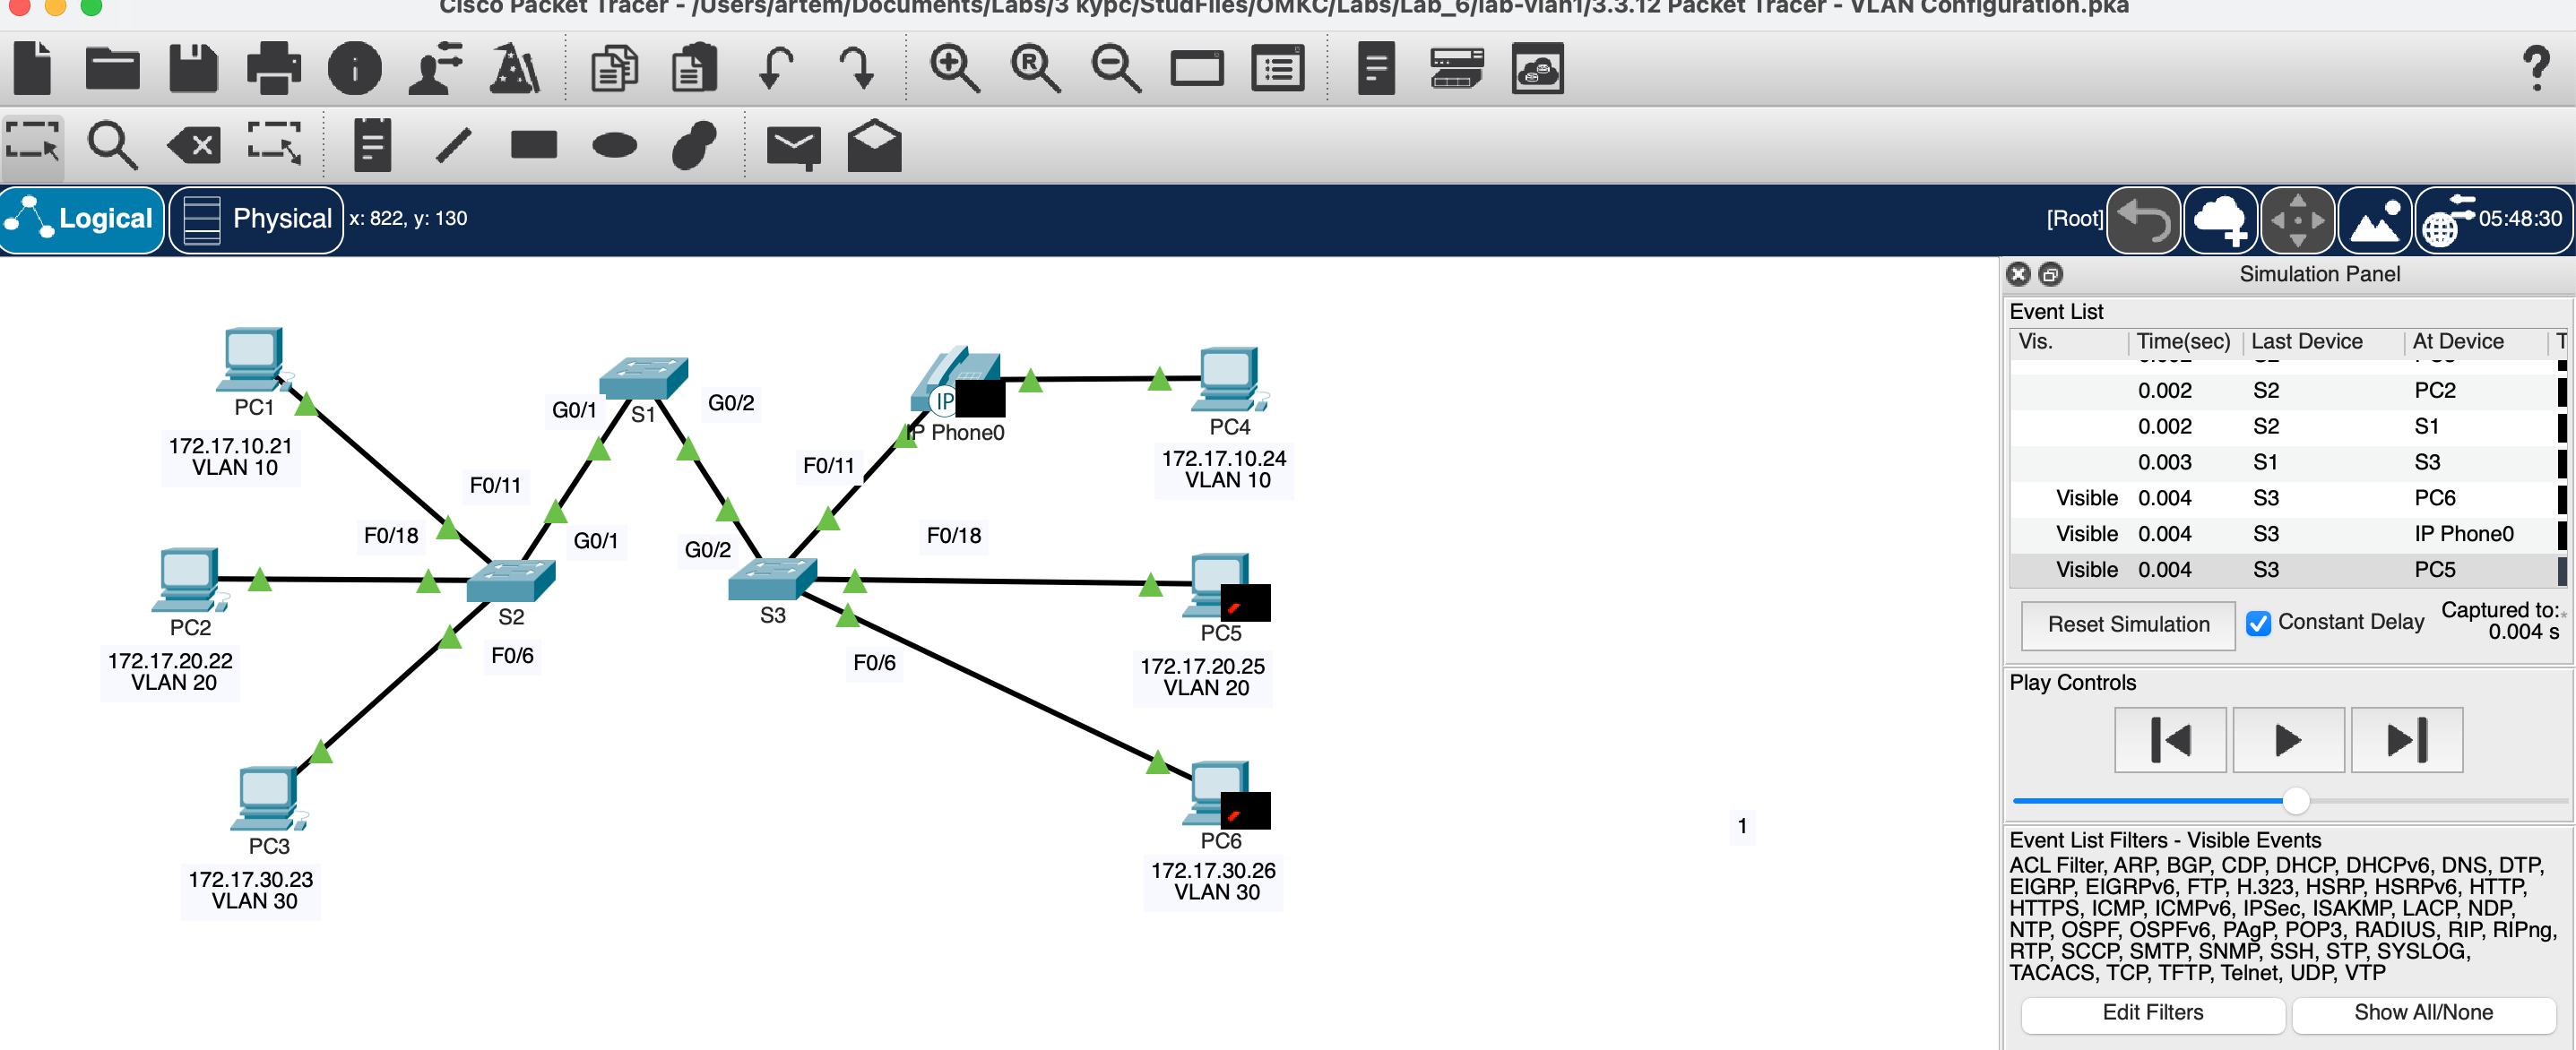
\includegraphics[scale=0.3]{pics/3.3.12_1.png}
                \end{center}

            \item Команды для настройки
                \begin{lstlisting}
en
conf t
vlan 10 
name Faculty/Staff
vlan 20 
name Students
vlan 30 
name Guest(Default)
vlan 99 
name Management&Native
vlan 150 
name VOICE
exit
exit
sh vl br
                    
conf t
int f0/11
switchport mode access
switchport access vlan 10
int f0/18
switchport mode access
switchport access vlan 20
int f0/6
switchport mode access
switchport access vlan 30
                \end{lstlisting}
            \item vlan настроены
                \begin{center}
                    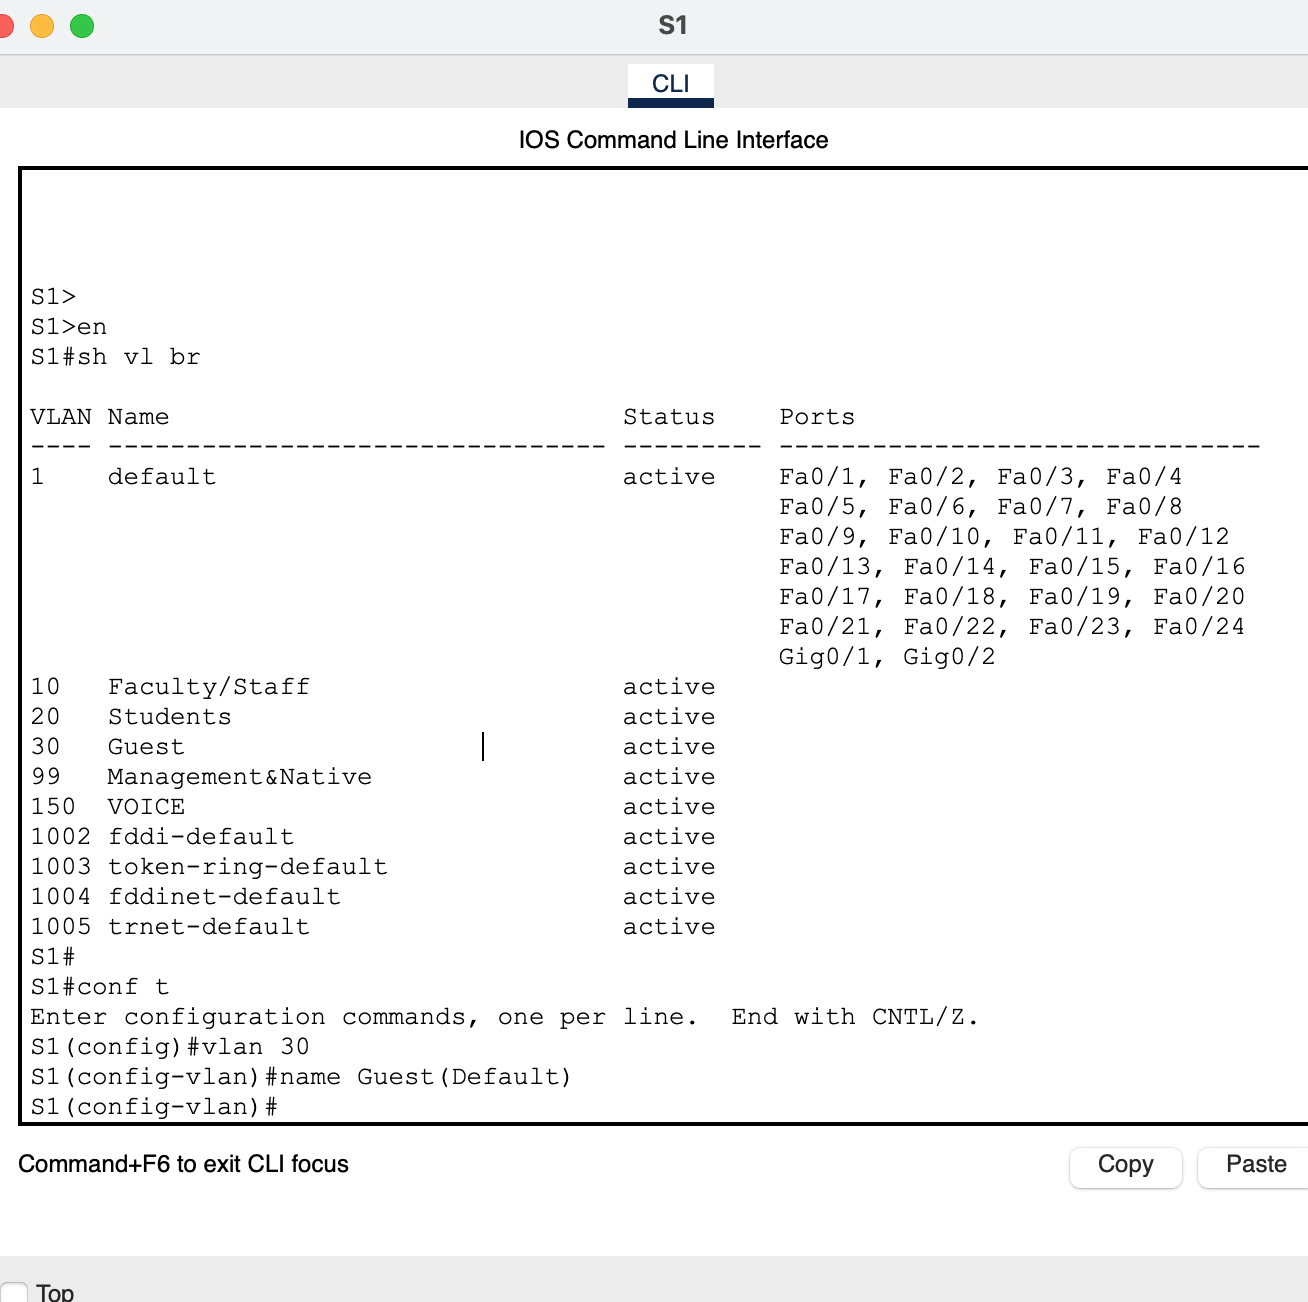
\includegraphics[scale=0.4]{pics/3.3.12_3.png}
                \end{center}
            \item \textbf{Успешно ли выполняются эхо-запросы при назначении портов доступа в соответствующие сети VLAN?}\par
                Нет, эхо-запрос выполняется не успешно. 
                \begin{center}
                    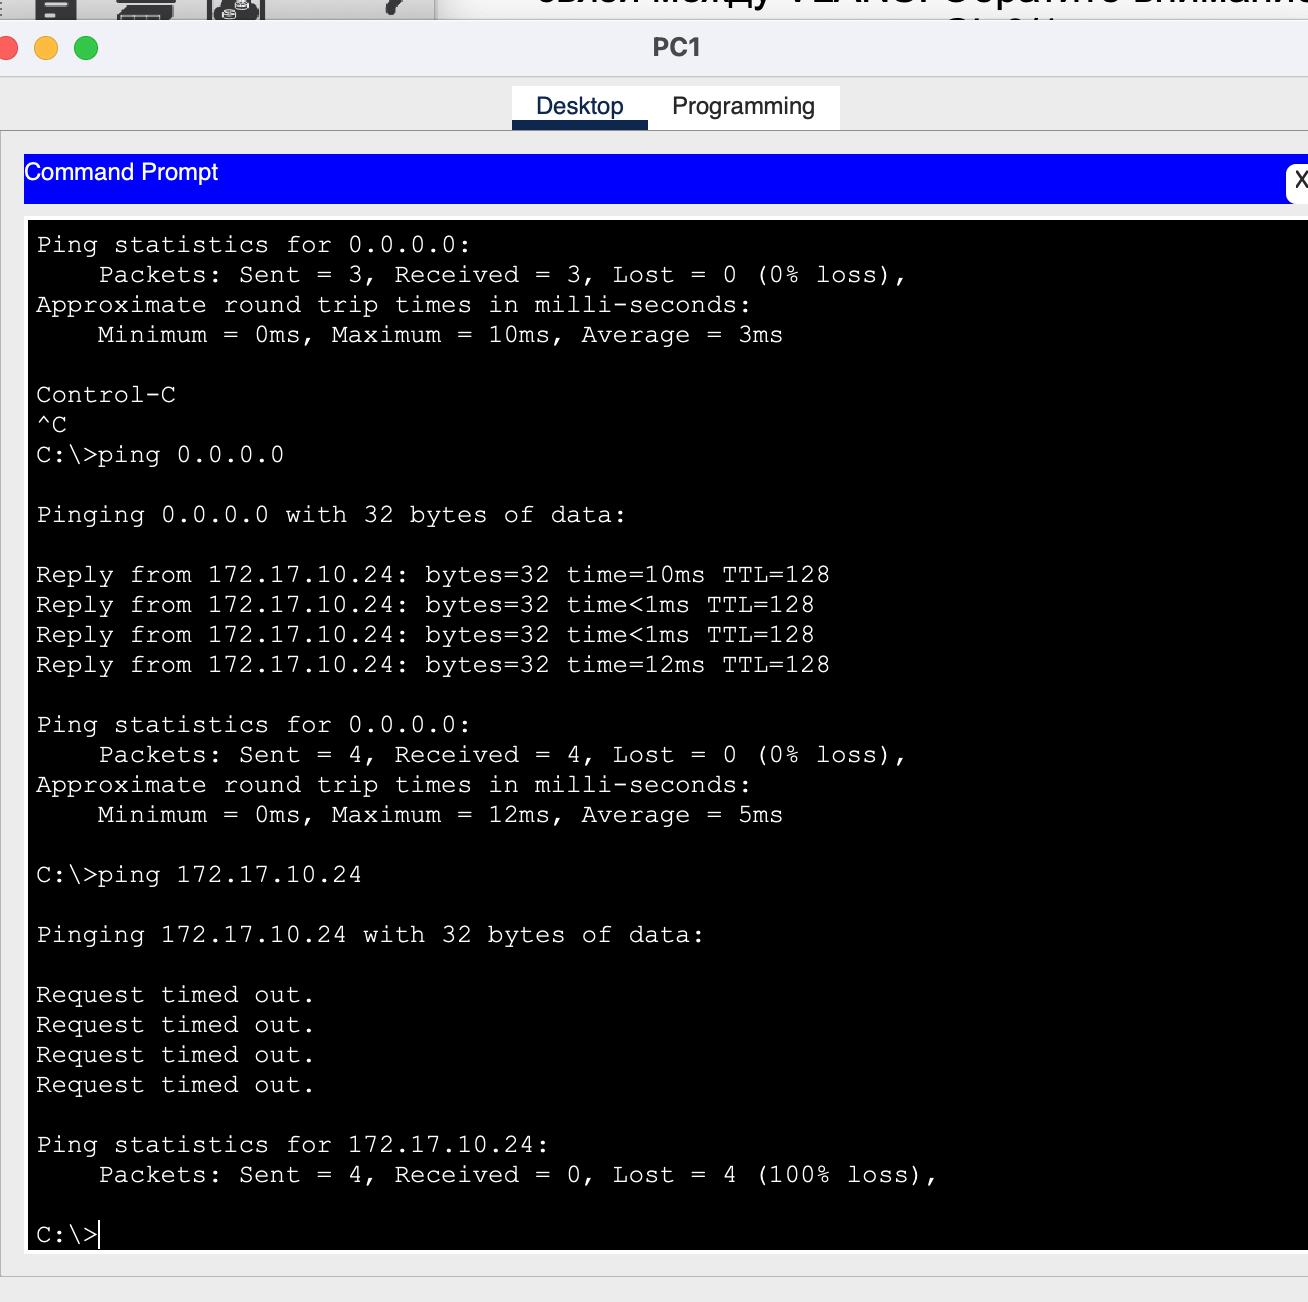
\includegraphics[scale=0.45]{pics/3.3.12_4.png}
                \end{center}

            \item \textbf{Что можно сделать для разрешения этой проблемы?}\par
                Для решения данной проблемы нужно настроить транки на гигабитных портах. А так же S1 коммутатор. 
        \end{itemize}
        \item lab 3.4.5
        \begin{itemize}
            \item Настройка trunk
                \begin{lstlisting}
switchport mode trunk
                \end{lstlisting}
            \item Настройка native vlan 
                \begin{lstlisting}
switchport trunk native vlan 99
                \end{lstlisting}
            \item \textbf{Почему при разных native VLAN на коммутаторах трафик все равно идет?}\par
                Это связано с тем, что любой нетегированный трафик в любом случае будет пересылаться в native vlan.
            \item \textbf{Каким активным сетям VLAN разрешено передавать данные по этому магистральному каналу?}\par
                1, 10, 20, 30, 88, 99
                
            \item \textbf{Почему порт G0/1 на коммутаторе S2 больше не назначен сети VLAN 1?}\par
                Так как данный порт переведён в режим Trunk.
                
        \end{itemize}
        \item lab 3.5.5
        \begin{itemize}
            \item Команды для настройки S2 и S3
                \begin{lstlisting}
en 
conf t
vlan 10 
name Red
vlan 20 
name Blue
vlan 30
name Yellow
exit
int range f0/1-8
switchport mode access
switchport access vlan 10
int range f0/9-16
switchport mode access
switchport access vlan 20
int range f0/16-24
switchport mode access
switchport access vlan 30
                \end{lstlisting}
            \item \textbf{Какие сети VLAN настроены на этих коммутаторах(S2, S3)?}\par
                Те же, что и на S1
            \item \textbf{В дополнение к VLAN по умолчанию, какие VLAN настроены на S2?}\par
                red, blue, yellow
            \item \textbf{Успешно ли выполнен эхо-запрос? Дайте пояснение.}\par
                Нет, эхо-запрос выполняется не успешно. Для решения данной проблемы нужно настроить транки на гигабитных портах. А так же S1 коммутатор.
            \item \textbf{Что будет результатом согласования магистрали между S1 и S2?}\par
                Поднимется транк между коммутаторами.
            \item \textbf{Каков режим и состояние этого порта?}\par
                Режим - auto, состояние - trunking.
            \item \textbf{Убедиться, что dpt отключен на 1 из 2х портов.}\par
                \begin{center}
                    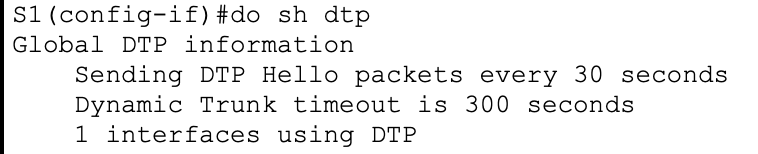
\includegraphics[scale=0.8]{pics/3.5.5_1.png}
                \end{center}
            \item \textbf{Какая сеть VLAN с нетегированным трафиком сейчас используется для этих магистралей?}\par
                Vlan 1
            \item \textbf{Какие сообщения вы получили на S1? Как бы вы исправили эту ошибку?}\par
                Несогласован native vlan. Нужно поменять на S2 и S3 native vlan.
            \item \textbf{Почему пинг не удался?}\par
                На S3 trunk не работает.
            \item \textbf{Какой режим и инкапсуляция на G0/2?}\par
                Вывод команды sh int tr был пуст. 
            \item \textbf{Что отображается состояние "Negotiation of Trunking"?}\par
                 Off
        \end{itemize}
        \item lab 3.6.1
        \begin{itemize}
            \item  Команды по настройке vlan
            \begin{lstlisting}
en
conf t
vlan 10
name Admin
vlan 20
name Accounts
vlan 30
name HR
vlan 40
name Voice
vlan 99
name Management
vlan 100
name Native
int f0/1
switchport mode access
switchport access vlan 10
int f0/2
switchport mode access
switchport access vlan 20
int f0/3
switchport mode access
switchport access vlan 30
            \end{lstlisting}
        \item SWA
            \begin{lstlisting}
hostname SWA
!
spanning-tree mode pvst
spanning-tree extend system-id
!
interface FastEthernet0/1
...
interface FastEthernet0/24
!
interface GigabitEthernet0/1
switchport trunk native vlan 100
switchport mode trunk
switchport nonegotiate
!
interface GigabitEthernet0/2
switchport trunk native vlan 100
switchport mode dynamic desirable
!
interface Vlan1
no ip address
shutdown
!
interface Vlan99
ip address 192.168.99.252 255.255.255.0
!
line con 0
!
line vty 0 4
login
line vty 5 15
login
!
end
            \end{lstlisting}
        \item SWB
            \begin{lstlisting}
hostname SWB
!
spanning-tree mode pvst
spanning-tree extend system-id
!
interface FastEthernet0/1
switchport access vlan 10
switchport mode access
!
interface FastEthernet0/2
switchport access vlan 20
switchport mode access
!
interface FastEthernet0/3
switchport access vlan 30
switchport mode access
... 
interface FastEthernet0/24
!
interface GigabitEthernet0/1
switchport trunk native vlan 100
switchport mode trunk
switchport nonegotiate
!
interface GigabitEthernet0/2
!
interface Vlan1
no ip address
shutdown
!
interface Vlan99
ip address 192.168.99.253 255.255.255.0
!
line con 0
!
line vty 0 4
login
line vty 5 15
login
!
end
            \end{lstlisting}
        \item SWC
            \begin{lstlisting}
hostname SWC
!
spanning-tree mode pvst
spanning-tree extend system-id
!
interface FastEthernet0/1
switchport access vlan 10
switchport mode access
!
interface FastEthernet0/2
switchport access vlan 20
switchport mode access
!
interface FastEthernet0/3
switchport access vlan 30
switchport mode access
!
interface FastEthernet0/4
switchport access vlan 10
switchport mode access
switchport voice vlan 40
...
interface FastEthernet0/24
!
interface GigabitEthernet0/1
!
interface GigabitEthernet0/2
switchport trunk native vlan 100
!
interface Vlan1
no ip address
shutdown
!
interface Vlan99
ip address 192.168.99.254 255.255.255.0
!
line con 0
!
line vty 0 4
login
line vty 5 15
login
!
end
            \end{lstlisting}
        \end{itemize}
        \item lab 4.2.7
        \begin{itemize}
            \item 
        \end{itemize}
        \item lab 4.3.8
        \begin{itemize}
            \item 
        \end{itemize}
        \item lab 4.4.8
        \begin{itemize}
            \item 
        \end{itemize}
        \item lab 4.5.1
        \begin{itemize}
            \item 
        \end{itemize}
    \end{enumerate}
\end{document}